\documentclass[12pt]{report}
\usepackage{WUthesis}
%\usepackage[latin1]{inputenc}
\usepackage{amsmath}
\usepackage{amsfonts}
\usepackage{amssymb} 
\usepackage{graphicx}
\graphicspath{ {images/} }
%\usepackage{listings}
%\usepackage{minted}
%\usepackage[revision]{revann}
\usepackage{tikz}
\usepackage{array}
\usepackage{subcaption}
\usepackage{caption}
\usepackage{soul}
\usepackage[per-mode=symbol]{siunitx}
\usepackage{physics}
\usepackage[style=numeric, url=false, isbn=false]{biblatex}
\addbibresource{thesis_bib.bib}

\newcommand{\comment}[1]{{\footnote{\color{green!40!black}#1}}}
\newcommand{\inlinecomment}[1]{{\bf\color{green!40!black} [\scriptsize #1]}}
\newcommand*\circled[1]{%
  \tikz[baseline=(char.base)]\node[shape=circle,fill=green!60!black!20!white, draw=green!40!black,,text=black,inner sep=0.2pt,font=\tiny\bf,minimum size=8pt] (char) {#1};}
\renewcommand\thefootnote{\protect\circled{\arabic{footnote}}}



\begin{document}


\title{An Analysis of Fireballs from Willamette's D6 AllSky Survey}
\author{Peter Joseph Gibson}
\thesissupervisor{Dr. Jed Rembold}

\maketitle


\newpage

\begin{center}
\textbf{Presentations and publications}

P. Gibson, Analyzing Fireballs from Willamette's D6 AllSky Survey, Oral Presentation at Willamette University, Research Seminar I: Status Report Presentation (December 2018)
\bigskip

P. Gibson, Analyzing Fireballs from Willamette's D6 AllSky Survey, Oral Presentation at Willamette University, Advanced Techniques in Experimental Physics: Senior Proposal Presentation (April 2018)

\bigskip
\end{center}



\begin{acknowledgments}
I would like to thank the following professors for their tremendous support and advice throughout my Willamette experience:
\begin{itemize}
    \item Dr.~Jed Rembold for teasing me and providing me with Hershey's Kisses as a consolation for his hate.
    \item Dr.~Rick Watkins for telling me "You got this!" in trying times.
    \item Dr.~Daniel Borrero, Dr.~Michaela Kleinart, Dr.~David Altman for their kindness and unwavering confidence in our graduating class.
\end{itemize}

I would also so like to thank the following people for helping me through countless homework problems, talking down my problems, and also picking on me when I deserve it:

\begin{itemize}
    \item Trent Jones for being a below par friend and an above par golfer.
    \item Jo Stensass for serving me all sorts of help along the way and providing a willingness to set me up for success.
    \item The wizards who answer questions on Stack Overflow and spend time editing Wikipedia to make it a more reliable resource.
    \item Not only to God but to Jesus.
\end{itemize}

Lastly, but perhaps most importantly, I would like to thank my mother and father for their unconditional love and for providing me with countless wonderful life opportunities such as the entirety of my college experience.  There is no argument that I would not be at this point without them.

\end{acknowledgments}

\begin{abstract}
\begin{flushleft}

\textbf{\textsc{\LARGE General Abstract}}

\vspace{0.2 in}

As fireballs, more commonly known as shooting stars, fly through Earth’s atmosphere at breakneck speeds, they emit light that can be observed on our planet’s surface. Willamette’s D6 AllSky Survey is a camera system that probes the night’s sky for these events which can be further utilized for large-scale analysis such as determining flux rates. Flux rates depict the number of events that occur per unit time per unit area. Because one camera system can only observe $<0.4\%$ of Earth’s total sky area, amateur astronomers hold a significant role in fireball observations. Their observations provide a robust data sample size that can then be used to gain a deeper understanding of the flux rates and property distributions of fireballs. While complex multi-camera professional systems currently exist, there is need for more economic, accessible, and versatile systems. We will discuss the feasibility of our current observational setup and how it compares to more elaborate existing systems.
\vspace{0.25 in}

\textbf{\textsc{\LARGE Technical Abstract}}

\vspace{0.2 in}

Fireballs, more technically known as bolides, are recognizable by the light they emit through ablation.  The D6 AllSky Camera was designed by Dr. Jed Rembold and Kyle McSwain as an alternative observation system for fireball research.  It is smaller, more portable, and significantly cheaper than most existing systems used by professional astronomers.  By measuring distributions of fireballs, primarily in the form of average flux, we aim to assess the feasibility of using the D6 AllSky Camera as opposed to other systems.  Due to poor weather and other unforeseen complications, our data sample was not sufficiently large enough to produce a confident average flux rate.  However the versatile framework established in this research will assuredly aid in the analysis of fireballs throughout further research.

\end{flushleft}
\end{abstract}

\tableofcontents
%\listoftables
\listoffigures

\chapter{Introduction}

Based on a rough estimate, there are about \num{10000} trillion ants, \num{7.6} billion humans, and a few million elephants in the world.
When considering this small\comment{these numbers are small?!} data set, one might come to the conclusion that there are more small objects in the world than there are large objects.
It so happens that this conclusion not only holds true on Earth, but it also holds true in our universe.\comment{I think you need a sentence to bridge these two.}
In our solar system, there is one star, eight planets, and an almost incomprehensible number of small rocks traveling through space. 

Similarly to distances in space, velocities of objects in space are of higher orders of magnitude than those observed on earth.\comment{So I get what you are going for here, but this is a convoluted sentence.}
For example, the Earth travels at approximately \SI{30}{\kilo\meter\per\second} while small rocks can travel between \SIrange{11}{70}{\kilo\meter\per\second}.  
The speeds of these rocks exceed the muzzle velocity of a bullet.\comment{probably want a citation here}
When we observe a meteor shower, we are witnessing a barrage of these bullet-like rocks.  
Fortunately for mankind, Earth’s atmosphere provides a protective shield consisting of a condensed array of particles.\comment{The start of this sentence is good but I don't like the end as much}
Condensed is a term being used in relativity to the vacuum of space in which these rocks spend the majority of their lifetime.\comment{I'd just bake this definition into the previous sentence}

As a rocky object travels through Earth’s atmosphere, it collides with particles and burns in a phenomena known as ablation.  
The result is a release of energy in the form of both heat and light.  
The objects, which ignite in a fiery ball are called fireballs.\comment{Careful here, technically fireballs are only the brightest meteors} 
For large enough fireballs, the light produced in ablation can be seen from the human eye as shooting stars.\comment{I'd remove this sentence and provide more context about the different magnitudes they might be seen at.}

By observing the photometric (visual) magnitude, duration, and other properties of individual fireball events, an observer can estimate impact energies and sizes of these near-Earth rocky objects.
Given a large enough sample size, observers can also determine the flux, or the number of events within a specific area per time, of fireballs of varying sizes and energies.\comment{Paragraph only has two sentences.}

While cameras set up by organizations such as NASA and the Spanish Meteor Network (SPMN) provide useful and precise measurements of fireball events, they lack flexibility and affordability.  
Often rendered immobile due to their connection to powerful computers, these systems provide only a small piece to the puzzle of fireball observation.\comment{What do you mean by small piece here?}
Any individual camera system can only observe up to around 0.03 percent of earth’s total sky.\comment{Oh, is this what you meant? I feel like this paragraph needs something more then.} 

This project aims to analyze the feasibility of the Willamette D6 AllSky camera, a new alternative camera system for conducting fireball research. 
Occupying about the same space as a traffic cone, this camera is easily transportable and can be replicated at a fraction of the price of the more expensive professionally used systems.\comment{Should be careful with language here, the camera itself is basically the same as in the other systems. The supporting infrastructure is what differs.}
By comparing flux rates measured through the analysis of data taken from Willamette’s D6 AllSky camera to more well-recognized systems, we will determine if our setup is a practical option for amateur astronomers interested in contributing to fireball research.\comment{Possibly break this sentence up and clean up the wording. Its possibly the most important sentence in your introduction, so don't skimp on it.}

This paper is broken up into several sections for ease of reading. Chapter 2 details useful information surrounding fireballs, their importance, existing research, and the theory necessary to calculate flux rates. \cite{trigo-rodriguez_2006_2007}\comment{Wait, why is this cited here? It seems super out of place...}

\chapter{Background}

Thanks to a protective atmosphere, Earth can withstand impacts from dust-sized to boulder-sized objects traveling faster than bullets without so much as a dent on Earth's surface.
While most of these near-Earth objects are extremely small and don't leave much of a trace, the larger objects can leave a light trail visible from Earth's surface as they burn up in our atmosphere.
In this chapter, we will discuss the classification of near-Earth objects, the camera system and equations we will use for our analysis, the existing photometry tools we have, along with other existing surveys.


\section{Description of Fireballs}

When considering types of near-Earth objects, many names come to mind.  
Asteroids, meteors, meteorites, and fireballs are often used interchangeably. 
However, there are several key distinctions between these objects.  
Asteroids are the largest of this group and are generally over $10$m in diameter \cite{meteoroidorbits}. 
These large objects are responsible for large craters that are visibly present on the moon.  
Meteoroids are anywhere between $10 \mu$m and $10$m and are drastically more common than asteroids.  

Meteoroids that pass through earth's atmosphere become meteors.
As meteors pass through the atmosphere, they begin to ablate, or release light.  
This phenomena happens because the interactions between the meteor molecules with the air molecules produce lots of energy, some of which goes into the production of light.
This light can be measured in terms of apparent magnitude.
Magnitude is represented on a $\log_10$ scale and dimmer objects are represented by high numbers while brighter objects are lower.  
If the meteor releases visible light below an apparent magnitude of $-4$ qualify as bolides, or fireballs.
For reference, Venus is a magnitude $-4.4$ planet while the dimmer Jupiter has a magnitude of $-2.1$.


If an object is massive enough to withstand the pressures of Earth's atmosphere and make it to the surface of Earth, it is classified as a meteorite. 
These are extremely uncommon, but provide valuable information about the rock's origin.
Figure \ref{jed} shows the relationship between these 4 objects.

\begin{figure}[ht!]
  \centering
  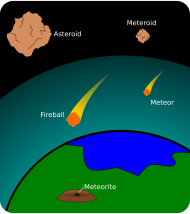
\includegraphics[scale=0.5]{images/jedmasterpiece.png}
  \caption{A depiction of near-Earth object classification.}
  \label{jed}
\end{figure}

We may further classify near-Earth objects into two categories: sporadic events and meteor shower events. 
Meteor showers occur when Earth's orbit crosses paths with the orbit of a collection of debris. 
Such collections often orbit large masses such as Jupiter or the sun \cite{trigo-rodriguez_2006_2007}.  
For example, the Perseid meteor shower has a highly elliptical orbit around the sun as seen in Fig. \ref{perceid}.  
A majority of the composition of these showers stems from the decomposition of comets throughout space.  

\begin{figure}[ht!]
  \centering
  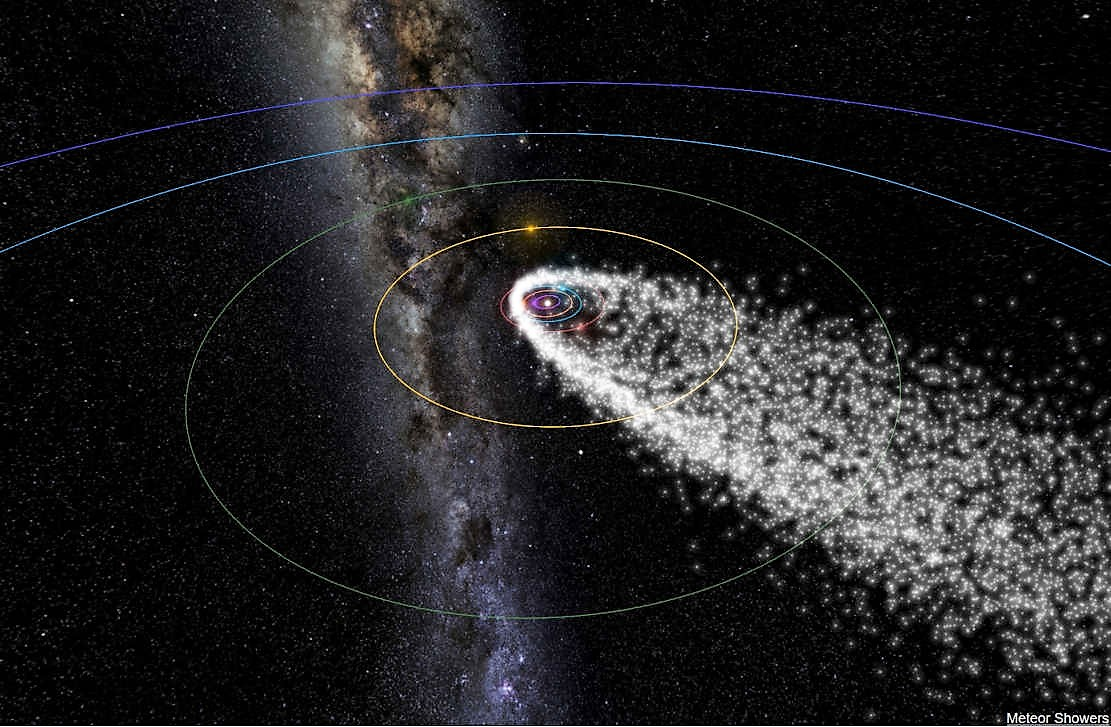
\includegraphics[scale=0.7]{images/persiod_shower.jpg}
  \caption{The Perseid meteor shower and its relation to our solar system.}
  \label{perceid}
\end{figure}

In contrast, there is debris in space that is not connected to any meteor shower. 
These are called sporadic events. 
Because gravity tends to bring objects together, we see mostly collections of debris.
However, when objects escape their collection due to other interactions (gravitational or electromagnetic), they still have a chance of colliding with Earth.

Studying these near-Earth objects can give us good estimates for how many objects you might expect to see pass through a given area of space within a specific amount of time. 
This measurement is called flux.
By determining flux, we can more accurately predict the likelihood of objects in space being hit by near-Earth objects. 
Although the case may have been an extreme one, the space satellite Olympus was struck and destroyed by a meteoroid during the Perseid meteor shower in 1993 \cite{threat}.
Additionally, given the relationships between the number of objects hitting earth per time for different objects, we can estimate the probability of extremely large impacts on earth.
These estimates, similarly to predictions surrounding volcanic or earthquake activity, give us insight into past events and help us foresee likelihoods of future events.








\section{The D6 AllSky Camera}

The Willamette University D6 Allsky camera was created in 2016 to capture the paths of fireballs throughout the night sky. 
The aim of the project was to create an economically feasible and easily mobile observational system.
By using a state-of-the-art camera system, a structure, some necessary reinforcement materials, and a programmable microcomputer, Kyle McSwain alongside Dr. Jed Rembold were able to get a functioning camera system \cite{mcswain_using_2016}. 
The camera resembles a Star Wars droid, and acquired its name from this inspiration.
This resemblence (paired with a little imagination) is shown in Fig. \ref{droid}.
The D6 Allsky camera is currently functioning properly and has been taking data since the summer of 2018.  
Below, we will discuss the composition of the D6 AllSky Camera while also highlighting what makes it significant.

\begin{figure}[ht!]
  \centering
  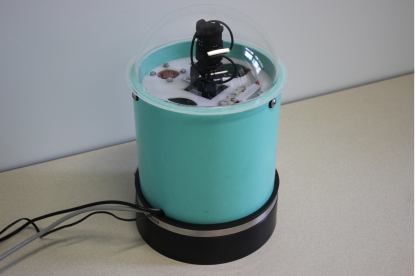
\includegraphics[scale=0.7]{images/allsky_camera.png}
  \caption{The Willamette D6 AllSky Camera (2016) \cite{mcswain_using_2016}.}
  \label{droid}
\end{figure}

\subsection{Composition}

The operational aspect of the D6 AllSky Camera is composed primarily of 5 different pieces: the camera housing, CCD camera, thermostat, digitizer, and the microcomputer (used to be raspberry pi).
The acrylic dome and PVC shell are both vital parts of our system. 
The dome itself is a transparent half sphere that sits on top of a PVC cylinder that holds the system together.
It acts as a protective layer between the camera and the outside environment.  
Without this feature, the camera would be subject to dew, bug contamination, and other undesired interferences.

The CCD camera is perhaps the most important feature of the camera.  
The Watec $902$H$2$ CCD camera uses a fish-eye lens to capture incident light from the night's sky.  
It was chosen due to its extremely high sensitivity and resolution \cite{mcswain_using_2016}.
While some fireball camera stations are composed of multiple high resolution, more narrow lensed cameras, the D6 AllSky system only contains one camera mostly for economic reasons.  
This camera was chosen in part due to its compact size, an important part of the highly valued versatility of our system. 
The camera is kept at a relatively constant temperature by a thermostat and a fan system. 
Because of its constant use throughout the night, the system itself can get very warm and therefore needs some thermal regulation.

The digitizer is the tool that allows us to transfer camera information to the microcomputer efficiently.  
The camera outputs analog signals which through the digitizer are converted to digital signals.
Through cable connections, the digitizer then sends the new output to the microcomputer where the initial analysis is run. 
The microcomputer takes the frames from the camera's running video and scans for systematic changes in brightness.
These changes then trigger the recording and storage of a new video, which is saved for further photometric analysis.
By combining these parts into one system, we are able to capture and catalog fireball events.

\subsection{Uniqueness}

While there are several similarities in the composition of our AllSky camera to existing systems, there are several key differences.
The most prominent of these are the size, versatility, and cost of our system.
Around the size of a basketball, the D6 AllSky camera is extremely compact.  
Not only is it small, but it only relies on a single power chord for power.  
Because of this, the camera can be relocated to any setting that has a power source.  
We should note that an external portable power source is a potential upgrade to this system that may take place in future creations.
Most other systems are rooted to extremely powerful computers that have little to no mobility as shown in Fig. \ref{immobile}.

\begin{figure}[ht!]
  \centering
  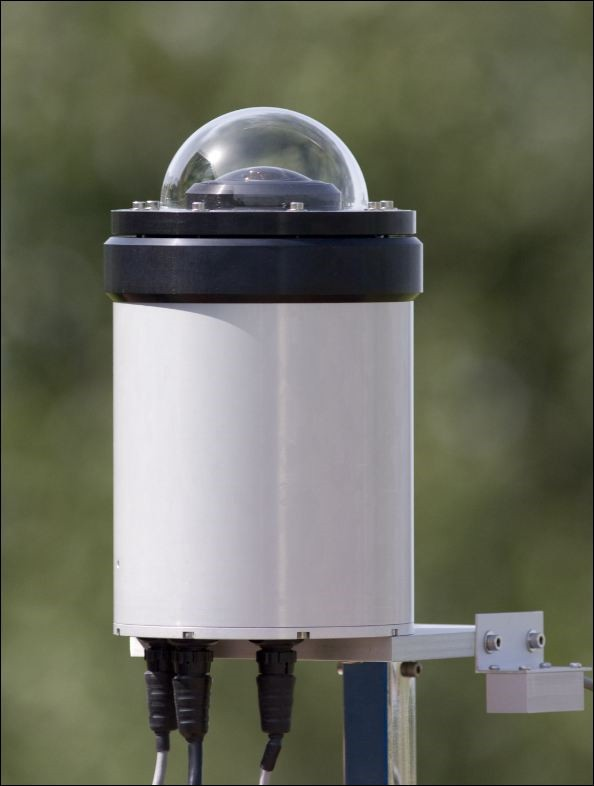
\includegraphics[scale=0.3]{images/othercam.jpg}
  \caption{An entrenched alternative AllSky camera.}
  \label{immobile}
\end{figure}

This presents issues related to being rooted in one location.
For example, if a tree were to grow near the camera, it would need to be chopped down or the entire system may need to be relocated.
With the lightweight and easily movable D6 AllSky camera, relocation is not a difficult process.

Most importantly, the D6 AllSky camera is a less expensive alternative to other fireball analysis tools.  
The ingenuity of running initial analysis on a microcomputer allows the D6 AllSky camera to cost a fraction of what professional systems cost.
Although large professional organizations produce copious amounts of wonderful data, in the field of fireball research, non-intensified systems outnumber intensified systems $2:1$ \ref{Molau}.  
Providing this cost efficient alternative could be a great way to expand the field of fireball research and in turn provide a better understanding of the near-Earth objects in our solar system.






\section{Photometry}
After collecting videos of potential fireballs, next comes the task of analyzing the videos.
Luke Russell, advised by Dr. Jed Remobld created a photometry program that allows us to get a calibrated intensity light curve for a given video of a fireball.
Simply running a fireball video through his interactive GUI allows us to access information about luminous properties of the fireball.
However, limitations to our photometry must be taken into account.
False positives, extinction, and other bothering problems must be accounted for while creating our fireball catalog.

\subsection{Existing photometry tools}
When running a video through the existing photometry script, the user must interact with the program.
After selecting a file to run through the program, the user must find the frame in the video which the fireball first becomes visible.  
Then, the user must left click on the fireball.
After this, the user must right click on a reference star with a known magnitude.
This step requires a bit of knowledge and will hopefully be automated throughout this project.
After selecting both of these and entering in the known magnitude of the reference star, the program will automatically track the fireball throughout the following frames.
By using Gaussian fits to the photometric data, the program is able to center its view on the fireball and determine its size throughout its path.
Throughout this process, the video also sums the photon counts for each fireball pixel for each frame.
This photon count gives us the magnitude of the fireball at a given point in it's path.
Doing this for each frame results in a light curve that shows the magnitude as a function of time.  
By using relations given in the Analysis section, we are able to calibrate the magnitude and from that calculate the intensity which yield the valuable light curve.
From this light curve, we can then move on to further analysis.

\subsection{Planes, \st{Trains} Bugs, and \st{Automobiles} Extinction}

\begin{figure}[ht!]
  \centering
  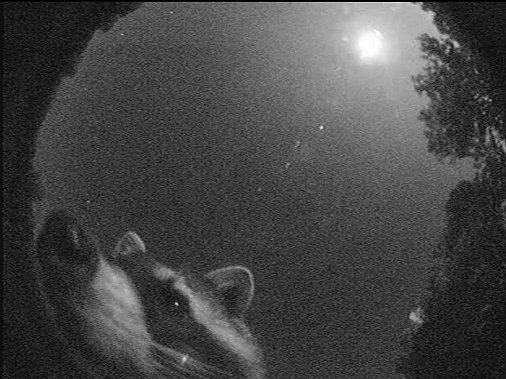
\includegraphics[scale=0.3]{images/racoon_cam.jpg}
  \caption{A fireball/raccoon hybrid.}
  \label{raccoon}
\end{figure}

While it is able to capture fireballs, the D6 AllSky camera still picks up a great deal of false positives.
In an initial sample of over $700$ videos, only $2$ of them contained real events.
The vast majority of the videos were of bugs crawling across the acrylic dome.
Because the bugs are illuminated by nearby light, they appear to be bolides traveling across the screen.
Many bugs are featured in several videos as they have a tendency to move, stop somewhere, and move again.
While this is somewhat problematic, we aim to implement several steps to limit the number of false positive bug cases.

In addition to bugs, airplanes, satellites, and iridium flares provide false-positive videos.
Their near-linear motion and bright presence are an instant trigger for the fireball detection.
This is a more difficult bug to fix when compared to the bug bug :).
These two cases are just small examples of false positives that result in difficult data to process.

\begin{figure}[ht!]
  \centering
  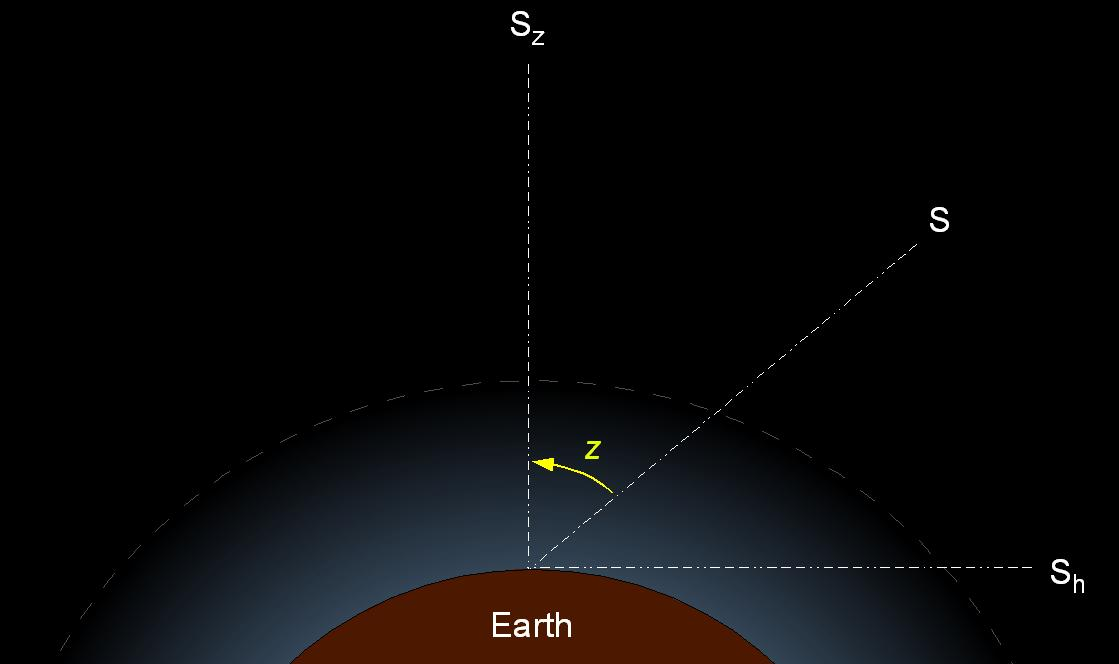
\includegraphics[scale=0.4]{images/extinction.JPG}
  \caption{A depiction of atmospheric extinction.}
  \label{extinc}
\end{figure}

A larger problem in data analysis stems from the phenomena of atmospheric extinction.
As shown in Fig. \ref{extinc}, we observe that when looking close to the horizon (S$_h$ in the image), light must travel through a larger volume of atmosphere than it does for an observation close to the zenith (S$_z$ in the image).  
Because the light travels through more atmosphere, more of the light is absorbed by gases or scattered by air particulates \cite{atmospheric}.
A prime example of atmospheric extinction is that of the sun. 
When directly overhead, the sun is at its brightest and one should never directly look into it.
However, close to the horizon, the sun appears more red and can be looked at directly.
Because a rising or setting sun's rays must travel through more atmosphere, they are scattered due to this extinction and become more comfortably visible.
Part of this project will include accounting for atmospheric extinction in a secondary photometric analysis script.






\section{Analysis}

\subsubsection{Parameters of Interest}



\subsection{Flux}







\section{Existing Surveys}
While amateur astronomers and low-budget systems capture useful information, larger professional systems act as a vitally important comparison point.
Individual events captured by an observer do contribute to the pursuit of knowledge.
However, a small camera system that cannot yield similar data to more professional surveys serves only a marginal amount of utility.
Cameras for AllSky Meteor Surveillance (CAMS), the SPanish Meteor Network (SPMN), and the Lincoln Near Earth Asteroid Research (LINEAR) program are examples of well-established existing meteor observing surveys.  
All of these programs are continuously acquiring data and adding their findings to existing databases.  
Nearly all of this data is widely available, and is available to the public online. 



\subsection{CAMS}
Funded by NASA, Cameras for Allsky Meteor Surveillance (CAMS) aims to verify minor meteor showers and trace them back to their existing parent comets \cite{jenniskens_cams:_2011}.  
The project was created by Peter Jenniskens and is based in California.  
The CAMS network is spread across 3 different locations and consists of over 60 cameras.
Each camera is has a relatively narrow field of view $~30\deg$.
Although they individually cover a small area, multiple cameras overlapping in field of view contribute to a large sky coverage. 
CAMS uses powerful CCD cameras to detect extremely dim meteors (up to around $+5$ mag).
By spreading their cameras across three separate locations, the CAMS research group can measure extremely precise trajectories of the incoming meteors. 
Similarly to the phenomena of trying to catch a baseball with only one eye open, confidently capturing a three dimensional trajectory of a fireball is extremely difficult when using only one camera.
Consisting of $3$ cameras located within $25$ miles of one another, as seen in Fig. \ref{trio} the CAMS survey have a median trajectory error of $0.31\deg$ and a median speed error of $0.53$ km/s \cite{jenniskens_cams:_2011}. 

\begin{figure}[ht!]
  \centering
  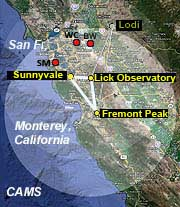
\includegraphics[scale=0.7]{images/CAMS_trio.jpg}
%   \setcaptioncitation{http://cams.seti.org/maps.html}
  \caption{The three CAMS network stations within a $50$ mile radius.}
  \label{trio}
\end{figure}

Accurate trajectories are particularly useful in back-tracing the motion of the meteor's orbit.  
The CAMS team has reduced over $320,000$ of these orbits \cite{seticams}. 
In addition to calculating orbits, CAMS also uses their precise velocity measurements to draw relations between speed and other properties. 
Figure \ref{fancyCAMS} shows the relationship between the apparent incident speed and peak magnitude.

\begin{figure}[ht!]
  \centering
  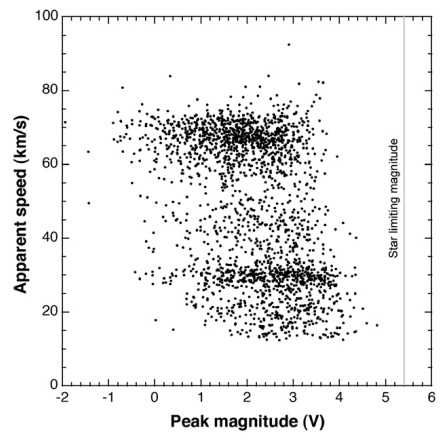
\includegraphics[scale=0.6]{images/CAMS_plot.png}
  \caption{Relationship between incident apparent speed and peak magnitude for CAMS data taken in November of 2010 \cite{jenniskens_cams:_2011}.}
  \label{fancyCAMS}
\end{figure}


Although the plot itself doesn't show a linear relationship, when considering the two subsets of relatively higher and lower incident speeds, we can see a general trend.
That trend shows that lower incident speed meteors tend to have slightly dimmer peak magnitudes. 



\subsection{SPMN}

The SPanish Meteor Network (SPMN) works extremely similarly to the CAMS project.  
It consists of $25$ observation stations located across Portugal and Spain \cite{trigo-rodriguez_2006_2007}.
Figure \ref{SPan} shows the approximate coverage of these stations along with some proposed locations (in green), from a satellite point of view.  

\begin{figure}[ht!]
  \centering
  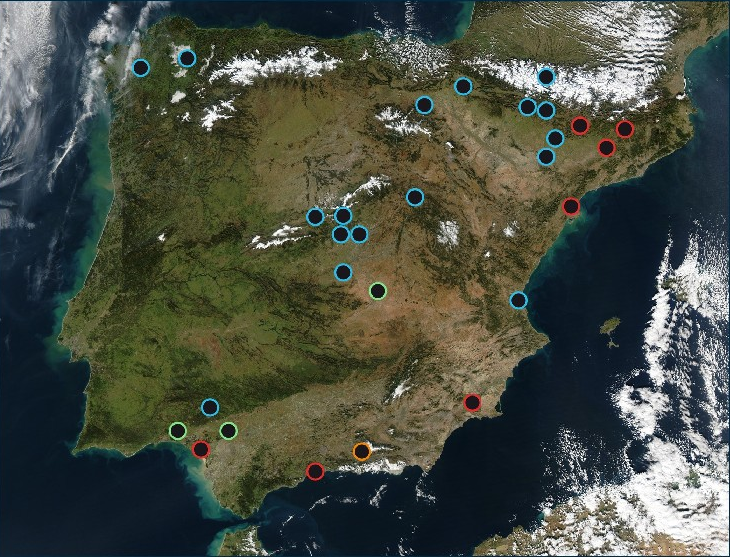
\includegraphics[scale=0.3]{images/satalite_of_love.png}
  \caption{Satellite view of the SPanish Meteor Network's sky coverage across $25$ existing and $3$ proposed observation stations  \cite{Spanish}.}
  \label{SPan}
\end{figure}

In addition to becoming the first organization in Spain to successfully calculate the orbital path of a meteor, this organization revolutionized fireball research by developing the first CCD AllSky cameras \cite{Spanish}.
These cameras are now in use all across the world.
While the SPMN and CAMS are extremely powerful research organizations, their study of meteors only slightly overlaps with the research being discussed in this paper.
Because of their high grade equipment, they are able to capture data from extremely dim sources.
Fireballs, quantified by a magnitude below $-4$, compose only a small fraction of the meteors analyzed by these organizations.
Fortunately, other organizations focus specifically on larger and brighter events.

\subsection{Other research groups}

There are a multitude of ways that one can attain information about a fireball.  
All the aforementioned surveys have employed the use of photometric data.
Peter Brown, a well renowned fireball researcher, took data from the Department of Defense and the Department of Energy space-based systems in geostationary orbits.
The original purpose of these systems is to detect signatures of explosions near earth's surface, but occasionally pick up false positives in the form of bolides.  
Because the systems detect the amount of power released, scientists such as Peter Brown can approximate the fireball's energy.
In a 2002 article published by \textit{Nature}, Brown estimated the optical energies of around 300 bolides.
From this data set and other existing data sets, Brown created Eq. \ref{browneq}, which relates bolide energy to the number of impacts on earth each year. 

\begin{figure}[ht!]
  \centering
  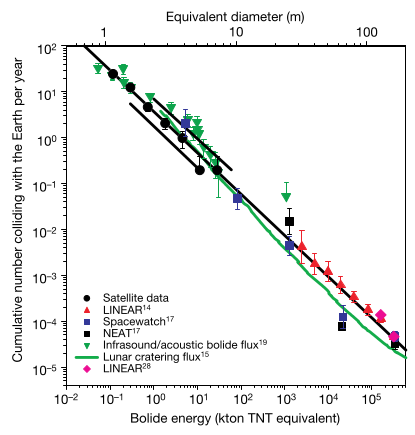
\includegraphics[scale=0.7]{images/flux_brown.png}
  \caption{A plot of bolide flux using an conglomeration of data \cite{brown_p_flux_2002}.}
  \label{powerlaw}
\end{figure}


Figure \ref{powerlaw} shows this relationship alongside data taken from many different research groups.  
In his research, Brown used existing assumptions (mentioned in the Analysis section) for the blackbody distribution and the velocity.  




%

\chapter{Methodology}

To calculate the flux of fireballs from our D6 AllSky Camera, we need to find the total observation area, time, and the total number of events.
In this section, we begin by describing in detail our methods for finding each of these properties.
Some time will be spend discussing obstacles such as camera fish-eye effect and cloud interference.  
Additionally, we will delve into the structure of our database: our fundamental tool for secondary statistical analysis.

\section{Calculating Total Observation Time}

Each night the D6 AllSky camera observes, a program is run on the controlling Raspberry Pi that logs important information throughout the night.
The observation log is a simple time-stamped text file that records what processes the system runs at various times in a given night.
For instance, the observation log contains when each observation run begins (when the camera is set up initially), when the camera begins its analysis, when a new event is detected, and when the analysis goes to sleep, along with potential warnings or error messages that might come up.

To calculate the total observation time, we run a Python script that searches for the time associated with the start of each new analysis.  
After this time is recorded, we continue down the list of information until we find the time associated with that observation run's end.  
By subtracting the two times, we find the total observation time for that specific night.  
Performing this same method in a loop throughout all of the nights allows us to find how much time we spent observing on a given night. 
By summing up the total time observed over each night, we can attain the total observation time over the course of our data collection period.

A depiction of a portion of an observation log and our time analysis table can be seen in Figure~\ref{obslog_time}.
Note that while the information row that contains "New Observation Run Started" sounds as if it represents the start time, we define our start time from the information row that states "A new night has arrived! Frame analysis beginning!".\comment{Should comment on why this is.}
End times are determined by the information rows labeled "Day has come.  Analysis going to sleep."

\begin{figure}[ht!]
  \centering
  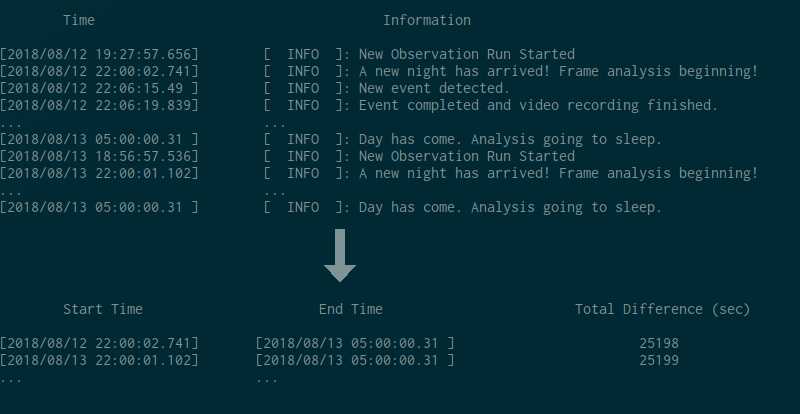
\includegraphics[scale=0.53]{images/obslog_time.png}
  \caption{An example observation log and the resulting time analysis information}
  \label{obslog_time}
\end{figure}

It is imperative that we save not only the total observing time over a given night, but also the start and end times. \comment{Is it important to comment about errors you find when doing this matching? Or if you throw away tiny portions where the camera was clearly being tested?}
This information is crucial for the next section, where we calculate the area of sky observed on a given night.

\section{Calculating Total Observation Area}

One of the most difficult problems we needed to address for this project was determining what area of the sky the D6 AllSky Camera observed each night.  
In an ideal world, our camera would be able to see all parts of the observable night sky, spanning across all horizons.  
However, due to optical limitations of our system and fisheye lens, this is not possible. 
Nevertheless, determining the flux is a primary goal of this project, and is directly dependent on observation area. As such it is vital we come up with a means to get a precise estimate\comment{This seems a bit of a paradox\ldots}. \inlinecomment{In this paragraph you were mainly focusing on the issue of us not getting the entire circle within our field-of-view, correct? Might want an image to better illustrate that.}

To make matters more complicated, while the use of a fisheye lens gets us more coverage of the sky, it also results in some distortion of the image.
These distortions generally get worse the further an object is from is from zenith (directly overhead).
An an example, imagine a square cloud located directly overhead.  
As that square drifts towards any given horizon, its size becomes smaller relative to you, the observer.\comment{Probably need more evidence or argument than this.}
The significance of this problem as related to our project stems from the fact that while $50\% $ of our camera's pixels may be covered by clouds, this doesn't necessarily mean that $50\%$ of the observable sky is covered.\comment{good, and well put.}
Therefore, we need some way of relating a given camera region to some observable distance.

To do this, we used observations of the Moon and various stars to calculate angular distance to pixel ratios for different regions of our camera.
This solution addresses the need to account for a camera fish-eye effect by assigning different fields-of-view to different pixel observational areas.
By correlating certain pixels with specific angular distances, we can analyze the available sky coverage by summing across all pixels.
To fully understand the methodology behind calculating the total observation area, one must understand how angular separation serves a role in area coverage.

\subsection{Angular Separation}

Consider two objects, both of which are visible to you, an observer.
One simple way to compare the two objects is by measuring the direct distance between them.  
An alternative way to compare the two would be to imagine two straight lines extending from your location to both objects.  
Because both lines are extending from the same location, we can calculate the associated angle between the two lines, known as the angular separation.
This angular separation may change as you move locations if the objects are nearby. However, if both objects are extremely far away, no small change in observer location will change the angular separation significantly.\comment{We use angular separation because we have no idea what radial distance separates the objects (generally). As such, we treat everything as being an equal radial distance away, and hence get the concept of the celestial sphere. And angles are a natural way to measure displacement on a sphere.}

We can apply this concept and principle to calculating angular distances between stars and other celestial objects.
By finding the angular separation across a given pixel, we attain a precise estimate\comment{this again} for angular coverage of the camera.\comment{only if we sum over all the pixels}
Assuming that the fireballs are ablating in our atmosphere at a given height, we can then apply our angular measurements to attain an observational surface area as desired.
It is easy to imagine this surface area used in flux calculations as the base of a cone, where the cone's point represents the viewer's field of view.\comment{But it is a rounded cone?}
Importantly,to calculate angular separation between objects, we need to first have a database of objects to compare.\comment{You really need a picture or pictures in this section.}

\inlinecomment{I think you need to revisit the idea that you want to use the known positions of stars and the Moon to serve as these calibration points before jumping into the next section.}
\subsection{Collecting a Star Catalog}

While the primary aim of the D6 AllSky Camera is to capture video footage of fireballs, it serves many other roles.\comment{This feels a bit awkward to me. It does these other things in an effort to better describe the population of fireballs.} 
Throughout the night, it takes several snapshots of the nights sky. 
The motivation behind this is primarily to check cloud coverage, but these images can store other important information.

Stars are visible in many D6 AllSky Camera's snapshots.  
The first step in creating a catalog of star information is recognizing stars within snapshots.  
We went about this by cleaning the image of hot spots, thresholding the image, and using the a \texttt{SimpleBlobDetector} to capture star locations.
All of these processes are coded and executed in Python.

\subsubsection{Hot Pixels and the Dark Frame}

Hot pixels are flawed pixels within a camera that always provide a significant positive photon count, even when the camera is exposed to complete darkness.
These pixels are problematic when trying to locate stars, as they don't represent any real physical object.
Fortunately, this source of error can be accounted for by taking an image while the lens of a camera is covered.  
This is called a dark frame, because the lens is not exposed to light.
Ideally the dark frame displays a black image, but most cameras will have a few hot pixels.
By subtracting this dark frame, represented by a 2-dimensional array of values ranging from $0$ to $255$, we are able to remove the hot pixel's effect from all other frames.\comment{An example would be nice.}

\subsubsection{Thresholding}

Once these hot pixels are subtracted from a given frame of interest, the next step is to enact some type of threshold.
In this case, a threshold represents a cutoff photon count\comment{Careful calling these photon counts. They are related but not directly proportional. Better to just call it pixel brightness.} for every pixel.  
If a pixel has a count that is lower than the threshold, that photon count is changed to zero, which is pure black.  
Alternatively, if a pixel has a count that is higher, the  count becomes 255, or pure white.  
Thresholding serves the important role of simplifying an image to a purely black and white, on or off type image.
It also remove some of the inherent error associated with photon counts.\comment{How are you justifying this? Or what do you mean?}
The necessary threshold for different images differed in accordance with the amount of surrounding light.
For the purposes of this project, we used an initial threshold of $140$.
If $140$ was not a sufficient threshold, this value was increased in increments of $5$ until the resulting image appeared to properly segment between open sky and clouds. 
For example, images that contained the Moon, a bright source that tends to wash out neighboring pixels, needed higher threshold values than images without.\comment{I'd like to see some images illustrating this here as well.}

\subsubsection{SimpleBlobDetector and Stellarium}

Next, we use the \texttt{SimpleBlobDetector} function from the \texttt{CV2} library to detect potential stars.
This function is able to read an image and scan for objects that meet your specified parameters.
Variable parameters include, but are not limited to, size (in pixels), circularity, convexity, and color.
In this instance, the color has a value of $255$.\comment{What about those other parameters?} 
When enacted, this function scans the picture and returns a list of detected locations centered on the object.
Using simple plotting functions, we can overlay these locations with the original image.

At this point, we have a list of potential object locations, but no foreseeable way of identifying the real ones.
As luck would have it, \textit{Stellarium}, a free astronomy software allows users to view a clear night sky from any point on earth at any time.
Additionally, this interactive software stores information about the stars' names and other important information.
By viewing \textit{Stellarium} and a D6 AllSky Snapshot and comparing the two, we are able to recognize which objects are real and which are false positives.\comment{"Why are there false positives? I thought we eliminates the hot spots?"}
Because each snapshot is labeled with the corresponding data and time, this method proved sufficient in identifying celestial objects from images.
A depiction of this process can be seen in Figure~\ref{star_recognition}.  
When comparing the two images, it should be clear that the objects numbered $17$, $16$, $19$, and $21$ correspond to Betelgeuse, Aldebaran, Capella, and Polaris. 
Also note that in the image, there are several recognized objects that don't have any celestial counterpart.
These are all false positives.
Similarly, there are cases in which the \texttt{SimpleBlobDetector} is not able to recognize an object that appears in a snapshot.
\begin{figure}[htb]
\centering
  \begin{tabular}{c|c}
    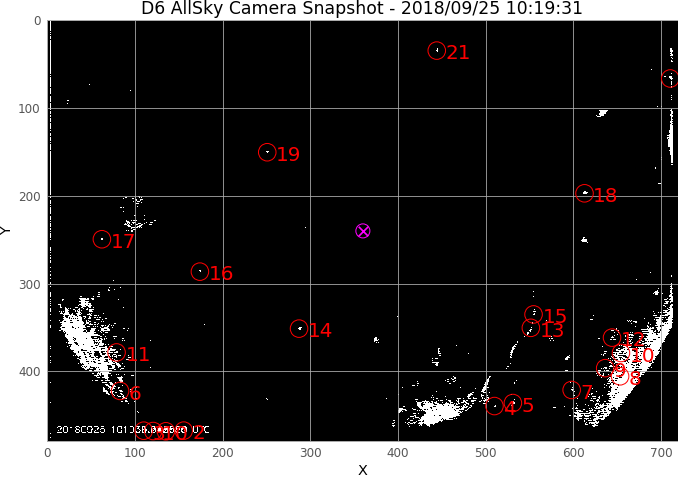
\includegraphics[width=.6\textwidth]{images/FourStarz_OneFrame.png} & 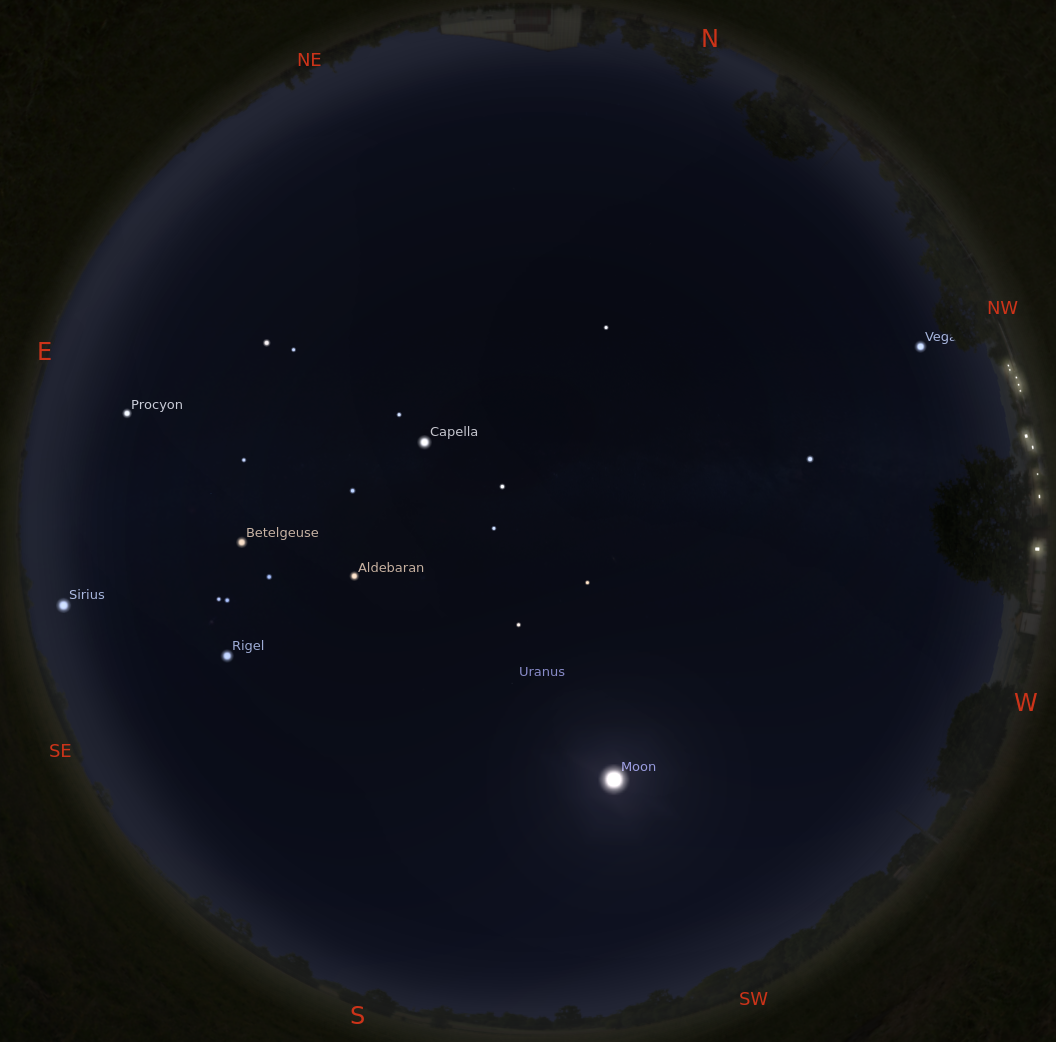
\includegraphics[width=.4\textwidth]{images/zoom_stellarium.png}
  \end{tabular}
  \caption{A D6 AllSky snapshot (left) alongside a Stellarium display (right)\inlinecomment{Please fix this image so the dark regions of the images align! Also, you need a much more robust caption explaining what is happening in each image. And you might want to zoom into Stellarium so its field-of-view roughly matches that of the image?}}
  \label{star_recognition}
\end{figure}

Once an object in a given frame is matched to a name, we used the coding library \texttt{Vizier}\comment{I'm actually not familiar with this. Is this a standard Python library or part of AstroPy?} to automatically look up the star's right ascension, declination, V-magnitude, azimuth, and elevation.  
This, combined with the star's pixel location, time, and reference file name\comment{What is this ``reference file name''?}, was added to our star catalog as a singular data row.

\subsubsection{Azimuth and Elevation}

Each star has several inherent properties such as magnitude, right ascension, and declination.  
The later two represent coordinates that locate a star on the celestial sphere.  
Other properties, such as a star's azimuth and elevation change over time and vary dependent on the observers location.  
These two properties indicate a star's position in the sky relative to an observer and act similarly to spherical coordinates.\comment{You really should comment or provide an image of what each one measures!}

Through finding the azimuth and elevation of a star, we can assign a star a 3-D coordinate value that lays on a unit sphere.  
Wwe can then calculate the angular separation between two 3-D coordinates by taking advantage of properties of the dot product:

$$ \vec{A} \cdot \vec{B} = |\vec{A}||\vec{B}| \cos{(\theta)} $$

where $\theta$ represents the angular separation between the two unit vectors.  
Because we know that both vectors representing star locations will fall on a unit sphere, their magnitude is $1$.
Using this knowledge, we may transform the above equation to:

$$ \theta = \arccos{(\vec{A} \cdot \vec{B})} $$

Given this formula along with information stored in the star catalog, we are able to calculate angular distance per pixel across different regions of the camera frame.\comment{Whoa, this is a jump. With this you can just calculate the angular separation between two points that we happen to see in our image.}


\subsection{Calculating Angular Areas}

The D6 AllSky camera is a versatile system and it's orientation can change slightly from night to night.
Because of this, there are several considerations that must be accounted for when calculating angular distance per pixel across different camera regions.
For example, if pixel $(10,10)$ has an angular separation per pixel of $0.10$ one night, if the camera rotates by $45 \deg$ we may read a different angular separation per pixel at that location. \comment{Should we though? Wouldn't the argument be that the camera should at least be rotationally symmetric?}
This is because the pixels may be representing a different area of sky upon rotation.
We have developed a method to account for this consideration.

\subsubsection{Comparing Objects from the same Night}

The star catalog stores information about celestial objects over the course of all observations.
Using constraints from the Time Analysis information (start time, end time, time elapsed), we can isolate rows within the star catalog from a specific night.  
After creating this subsection, we can then use our described method to calculate the angular separation per pixel for every combination of two objects.\comment{I'm confused. I don't feel like you have made clear how this angular separation per pixel is calculated yet?}
One might question where the data behind this angular distance per pixel should be located.
After all, there are two different object locations used to calculate the value.
Our strategy was to locate the point in between the two objects.  
Figure~\ref{starcombos} depicts these combinations along with the locations of the angular separation per pixel represented as white dots.

\begin{figure}[ht!]
  \centering
  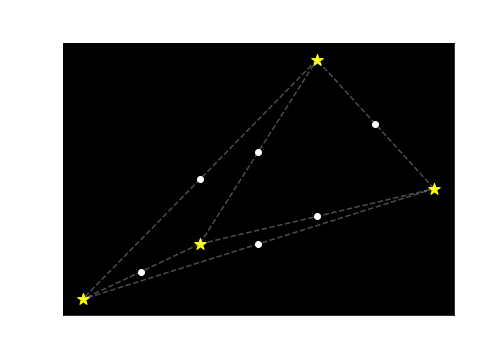
\includegraphics[scale=0.70]{images/star_combinations.png}
  \caption{A simplified depiction of angular distance per pixel locations\inlinecomment{Clarify what you mean by this.} (white dots) given a set of objects (yellow stars).}
  \label{starcombos}
\end{figure}

Figure~\ref{starcombos} gives a general depiction of our method on a much smaller scale.
Note that when comparing objects from this subsection of the star catalog, we are not limited to only comparing different stars.
As an object moves throughout the night sky, its azimuth and elevation change along with its pixel location.
We can thus treat each individual observation as a unique object, even comparing between the same object at different times throughout the night.
This creates many more combinations than if we were to only consider unique stars.

After calculating all potential angular separation per pixel values alongside their location information, we may move on to calculating average angular separation per pixel in different camera regions.
For the sake of simplicity and practicality, we split up our $720 \times 480$ pixel camera frame into $40 \times 40$ pixel squares.\comment{From a coding point of view, this wasn't really necessary. Why did we really do it?}
All angular separation per pixel measurements located inside a given square were averaged over to determine that square's value.
% Delete this picture and following sentence.  Replace with a more descriptive picture of the process, not the results.  Save for data section!
Figure~\ref{colorful2} shows the resulting average angular separation per pixel for different squares in our camera frame.\comment{Given your comment in the code. Is this the final version or the version that still needs fixed?}

\begin{figure}[ht!]
  \centering
  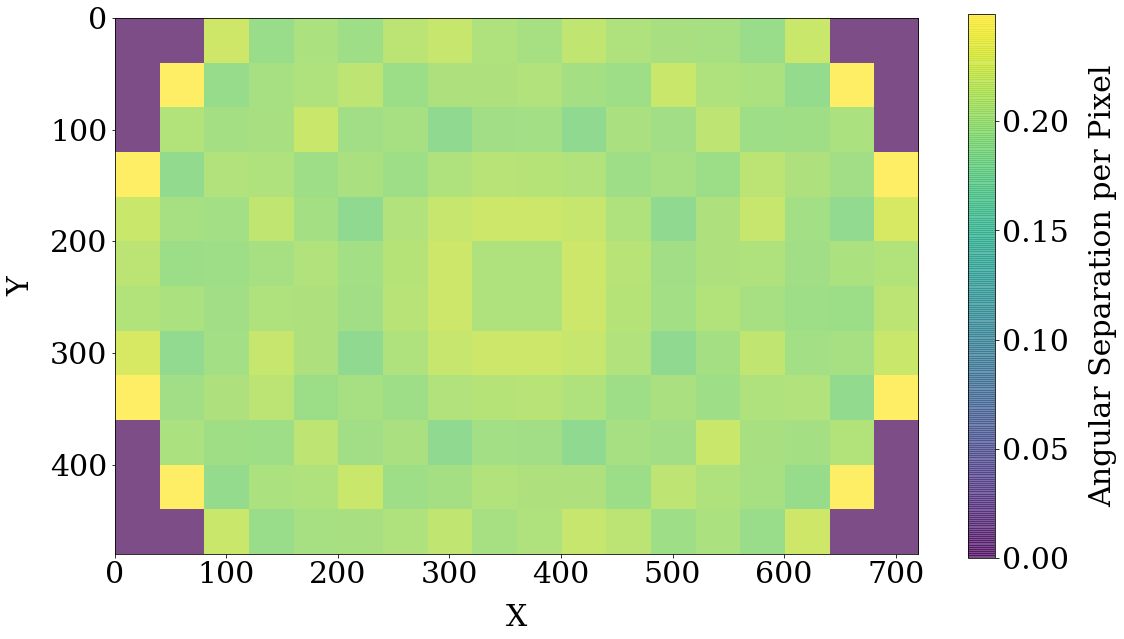
\includegraphics[scale=0.35]{images/boxes_colored.png}
  \caption{Average angular separation per pixel for different camera regions. \inlinecomment{Again, you need more robust figure captions. Also, did you ever talk about rotating the points?}}
  \label{colorful2}
\end{figure}


\section{Calculating Cloud Coverage}

The D6 AllSky Camera does not always remain outside.
For the protection of the system as well as for saving power purposes, the camera is only placed outside during nights where observation conditions are promising.\comment{That shouldn't remain that way forever though. The intent is clearly to have it outside all the time in the end.}
Some nights, the sky is clear throughout the entire night, while others are partially cloudy.\comment{Actually, given the direction you went with this, why even mention the above?}
Because we cannot see or properly analyze fireball events that happen behind clouds, we cannot count cloudy regions as observable areas.
As mentioned previously, the D6 AllSky Camera takes several snapshots of the night sky systematically throughout an observing session.
Specifically, it currently takes images every $30$ minutes.
By using thresholding, we have seen how we can determine which pixels qualify as not observable areas.
The threshold value that we used in this step was a photon value of $90$.\comment{Why does this threshold differ from the one earlier?}

Unfortunately, some pixels that fall within a broad cloud area are not recognized through this process.
The solution to this problem lies in the \texttt{CV2} functions \texttt{MORPH\_CLOSE} and \texttt{MORPH\_ERODE}.\comment{These are more any binary image functions that CV2 specific}
The first of these functions fills in regions of empty space that are next to filled in space.
This is helpful in closing gaps between pixels that represent clouds.
However, because the edges of the clouds are expanded in this process, we must subsequently perform a \texttt{MORPH\_ERODE} that works in the opposite fashion.
Once a hole is completely closed, there is no space within a cloud for the eroding function to open up, hence providing a satisfying answer to the cloud predicament.\comment{You should reference the image earlier for a visual to better understand what you are trying to eliminate.}

After this successful threshold and subsequent closing/eroding process is complete, the next step is implementing the relationships between pixels and angular distance as seen in Figure~\ref{colorful2}.
By assigning the correct regional angular separation per pixel value to each pixel within a cloud, we are able to estimate the angular area that cloud covers.
Figure~\ref{colorclouds} shows the processes taken in calculating the area occupied by clouds.
Note that both a filling and eroding function was used to attain the lower left image.
The observable area during that time is the cloud coverage subtracted from the total observation area.


\begin{figure}[ht!]
  \centering
  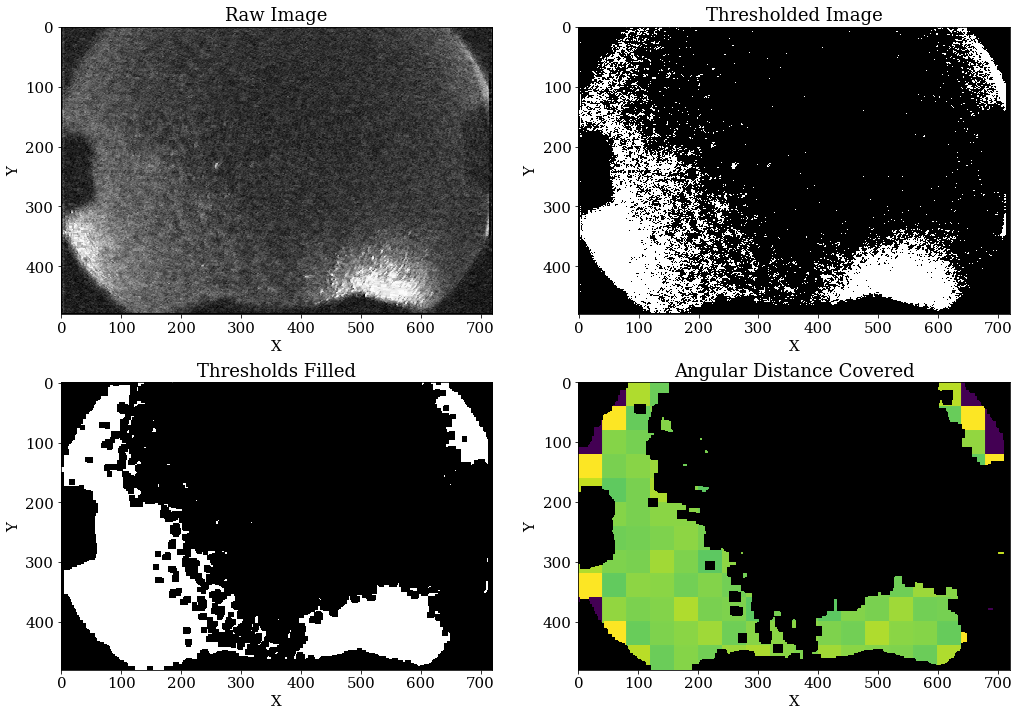
\includegraphics[scale=0.4]{images/Cloud_analysis.png}
  \caption{The processes behind determining the area of cloud coverage.\inlinecomment{Way more robust caption. This is arguably the most important image of your analysis section. Don't chince out on it!}}
  \label{colorclouds}
\end{figure}

This process is performed for each snapshot.
In creating our average area observed calculations, we assume that the sky retains that same amount of cloud coverage for the $15$ minutes prior to and $15$ minutes after the snapshot.
While this isn't precise down to the exact minute, over many observations, the number of over-estimations and under-estimations should average out and yield an accurate observational area.























 

%\chapter{Data}

Because there is intrinsic variability in the number of near-Earth objects colliding with Earth's atmosphere from night-to-night, a sufficient data sample plays a vital role in estimating an average flux.
This chapter details our data sample, specifically with respect to our time, observable area, and fireball distributions.  
To assess the overall capabilities of our system, we also delve into the data behind our star catalog, previously used for total observable area calculations.  
While this chapter provides the raw data samples and overall distributions, a further analysis and interpretation of the data can be found in Chapter 5.

\section{Time Distributions}

The D6 AllSky Camera does have a protective shell, however it is not always placed outside for nightly observations.
Due to Oregon's climate, we often leave our observation system inside.
There have been a total of $221$ days between August 27, 2018, the beginning of Willamette's academic year, and May 6, 2019.
Out of those $221$ days, we have been able to observe for \hl{$34$} nights, for a total of \hl{$291.87$} hours.

Once placed outside to observe, the D6 AllSky Camera begins taking observation when the sky is dark enough to take videos of without fear of over-saturation.
As the sky gets brighter when sunrise approaches, the camera automatically shuts off, ending the observation session.
This brightness constraint means that the total observation time changes from night-to-night.
We observed for an average of \hl{$8.584$} hours per night.
The shortest observation session lasted \hl{$7$} hours while the longest lasted \hl{$11$} hours.


\begin{figure}[ht!]
  \centering
  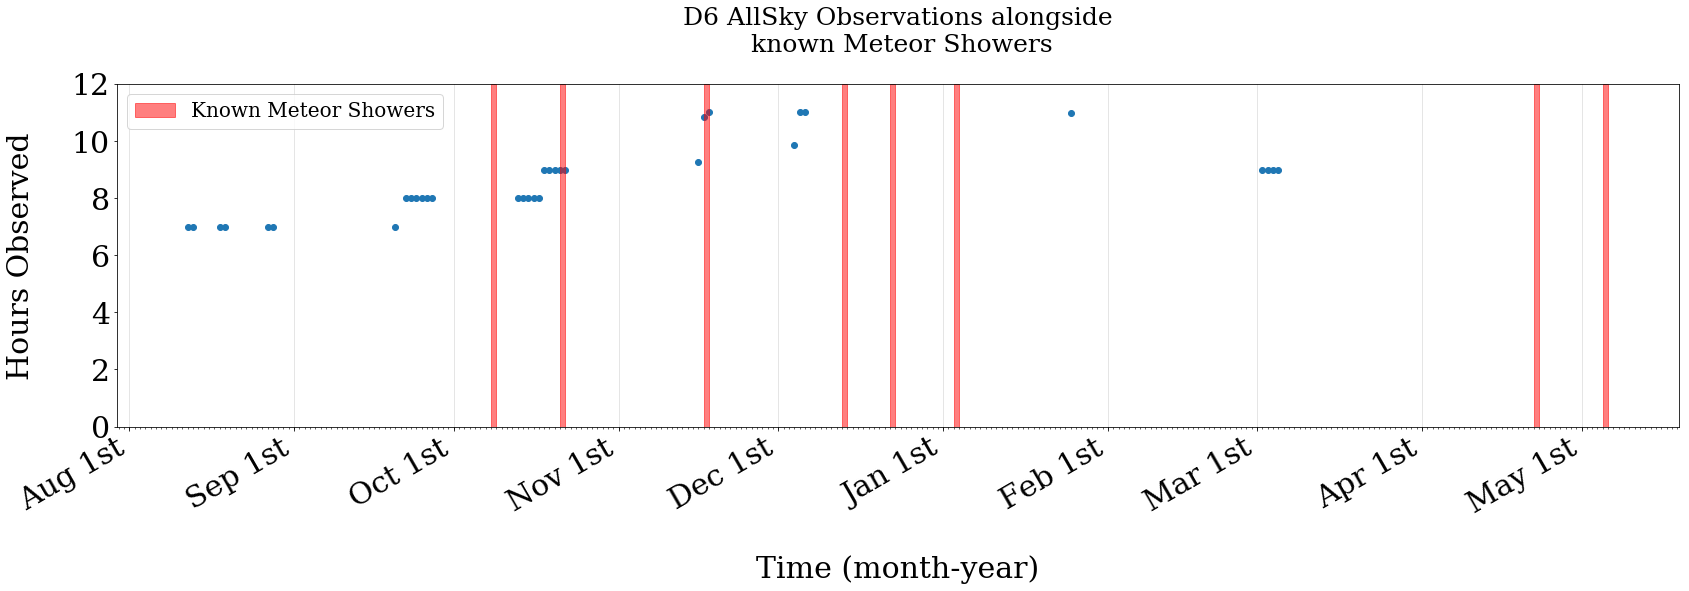
\includegraphics[scale=0.25]{images/nights_observed_with_meteorshowers.png}
  \caption{A plot of all D6 AllSky observation dates and recognized meteor showers within the $2018-2019$ academic calendar year.}
  \label{dateplot}
\end{figure}


Figure \ref{dateplot} displays the individual nights that we observed throughout the academic calendar. 
In addition to plotting our observation dates and that sessions total observing time, we have indicated dates of meteor showers visible in Salem, Oregon.  
During the months of October and November, we observed on nights of the Orionid and Leonid showers respectively.  
% Insert smooth transition




\section{Coverage Distributions}

As described in the methodology section, to calculate the angular distance per pixel for a given location, we needed two different celestial object measurements.
By taking the angular separation between the two, we designated the ratio to their respective midpoint.  
In total, we used \hl{$2638$} comparisons to create our angular separation per pixel data-set.  
Figure \ref{angperpix1} shows all of these points, each colored with their respective angular separation per pixel ratio.  

\begin{figure}[ht!]
  \centering
  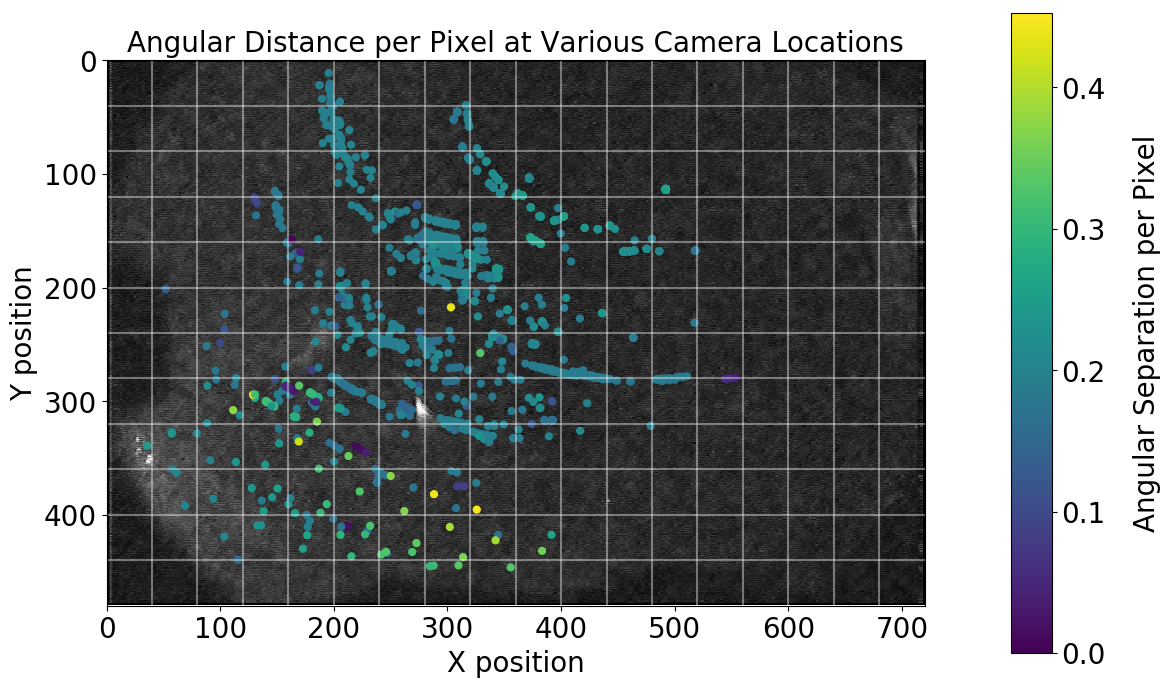
\includegraphics[scale=0.4]{images/angular_distance_at_various_locations.png}
  \caption{A plot of angular separation per pixel measurements from celestial comparisons.}
  \label{angperpix1}
\end{figure}

One may note that Fig. \ref{angperpix1} shows many data points, but they do not span the entirety of the camera field. 
There are many regions with no data points.
Because has a view that is symmetric about the azimuth, we rotated all of our data points by a fixed quantity and appended them to the current data set.  
This assumption of azimuthal symmetry allowed us to attain a more robust data sample without sacrificing data quality.
By rotating and appending in sequences of $5\degree$ in a full unit circle, we were able to increase the number of data points by a magnitude of \hl{$71.53$}.
From this point we were able to then bin the data and create Fig. \ref{colorful}.


\begin{figure}[ht!]
  \centering
  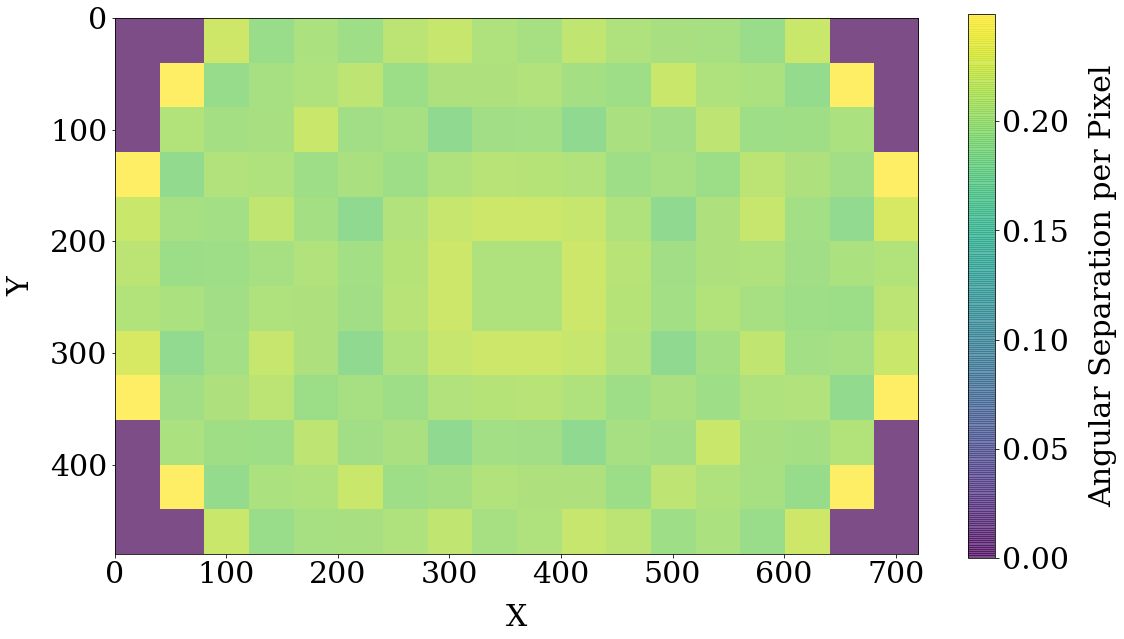
\includegraphics[scale=0.35]{images/boxes_colored.png}
  \caption{Average angular separation per pixel for different camera pixel regions.}
  \label{colorful}
\end{figure}

As described in the Background chapter, we used our measured solid angles for each region to calculate individual rectangular pyramid-created sky areas at a fixed radius of \SI{11.4}{k\meter}
Our measured total areal coverage was \hl{$->$} \SI{58974.88}{k\meter}$^2$ \hl{$<-$}.

As some nights were cloudy and others clear, the observable area value fluctuated in time. 
Figure \ref{time_area} depicts both the total observation time and the average observable area for each of our observation months. 

\begin{figure}[ht!]
  \centering
  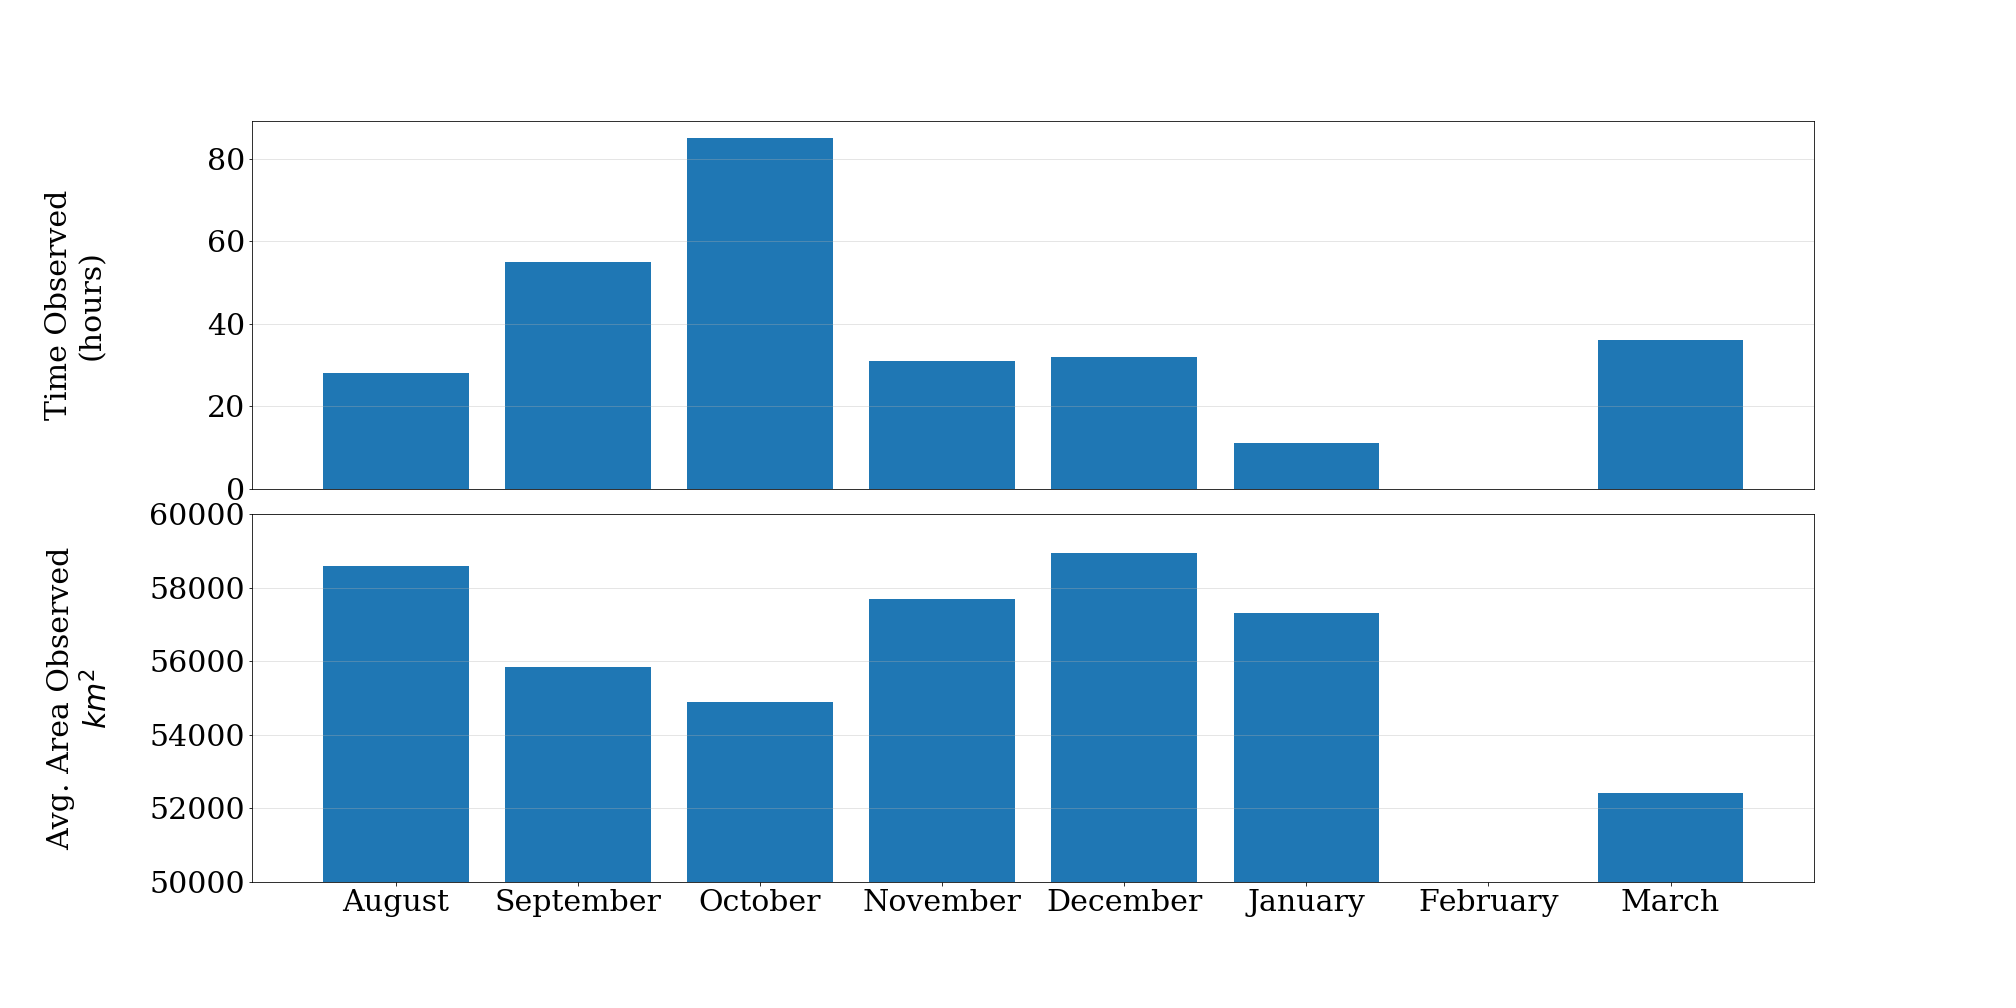
\includegraphics[scale=0.25]{images/time_vs_areaobs_plot.png}
  \caption{A plot of total observation time and average observable area for each month.}
  \label{time_area}
\end{figure}

Our average observable area across all observations was \hl{$->$} \SI{56012.03}{k\meter}$^2$ \hl{$<-$}.
This value, along with our total observation time and number of events will be used to determine the overall average flux.
% Insert smoother transition than this ^


\section{Detected Fireballs}

In total, the D6 AllSky Camera captured a total of \hl{$1095$} videos.  
Of those \hl{$1095$}, only \hl{$6$} were identified as real fireballs.
A depiction of the locations of these fireballs can be found in Fig. \ref{fireball_locs}.  

\begin{figure}[ht!]
  \centering
  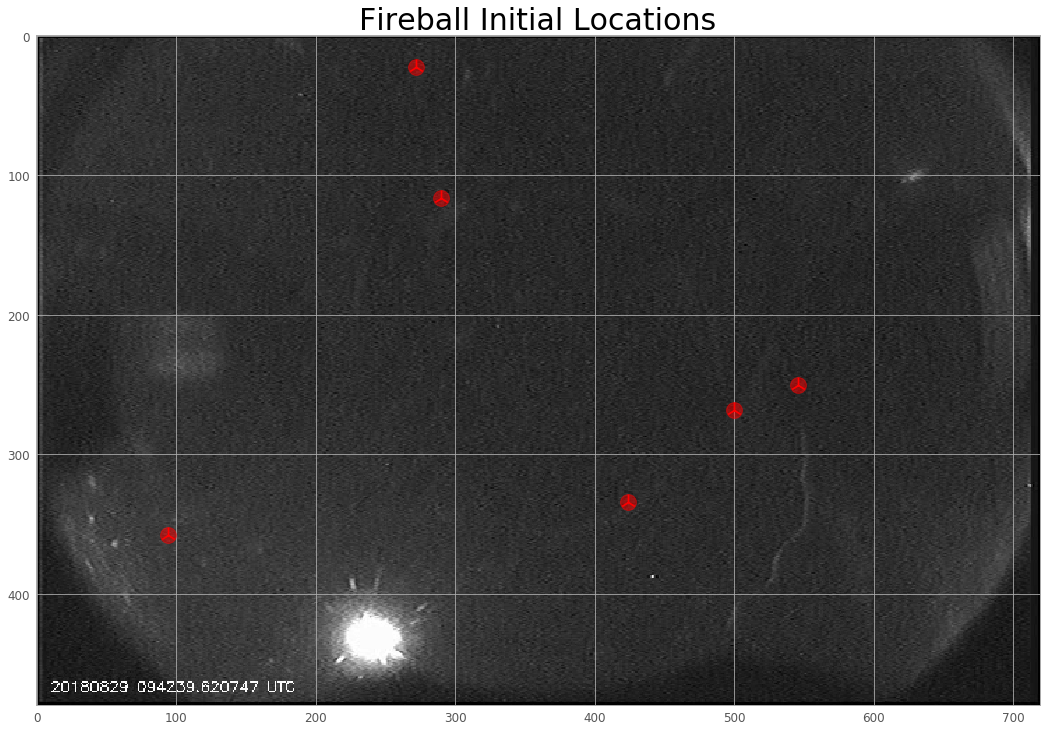
\includegraphics[scale=0.25]{images/fireball_initlocs.png}
  \caption{The initial pixel locations of all detected fireballs.}
  \label{fireball_locs}
\end{figure}

Of the \hl{$6$} fireballs, $3$ were found within $24$ hours of the Leonid meteor shower while $1$ more was found during the Orionid meteor shower.  

Unfortunately, the GUI program used to analyze fireball properties was unable to work on each of these cases.  
Therefore, we will have to wait for updated data on the property distributions of our catalogued fireballs.


\section{Camera Capacities}

As described in Chapter 3, the star catalog consists of recognized stars from the D6 AllSky Camera's snapshots.
In a catalog containing a total of \hl{$317$} rows we observed an average of \hl{$1.396$} stars per snapshot containing at least one star.
In total, the system took \hl{$1642$} snapshots, and \hl{$279$} of them contained celestial objects (stars or the moon).  
Within those \hl{$227$} videos, we captured information on \hl{$13$} unique objects.
Of these objects, the brightest had a Vmag, or apparent magnitude of $2$.  
This star is Alpheratz.  



%\definecolor{LightCyan}{rgb}{0.88,1,1}
\newcolumntype{g}{>{\columncolor{LightCyan}}l}


\chapter{Conclusion}

Calculating average flux only depends on three variables. 
Although this calculation appears simple, estimating an average observational area can extremely difficult. 
Through establishing a versatile method for calculating observable sky area, we can now estimate the D6 AllSky Camera's average flux and compare it to other systems.
As of this point, our data sample is too small to make any conclusive claims.  
There are still steps that need to be taken to truly assess the feasibility of using the D6 AllSky Camera in fireball research.  
This section will detail some of our self-assessed points of critique as well as shed light on some possible future research directions.

\section{Results}

After attaining the number of events, total observation time, and average observational area, we found that the D6 AllSky Camera had an average flux of \hl{$3.86 \times 10^{-7}$ hr$^{-1}$km$^{-2}$}.
Table \ref{table1} displays this value alongside the values that contributed to our flux calculation. 
As a point of comparison, Dr. Jed Rembold measured an average flux rate of $1.09 \times 10^{-7}$ hr$^{-1}$km$^{-2}$ when studying meteor impacts on the moon. 
The moon and earth are inherently two different objects with different gravitational effects.
However they have similar locations with respect to our solar system, implying that their average flux rates should share some resemblance.
The fact that the D6 AllSky Camera's fireball flux rate is of the same order of magnitude as research in the same field, we remain cautiously optimistic about the feasibility of our camera system.



\begin{table}[ht]
\setlength\extrarowheight{5pt}
\centering
\begin{tabular}{l|gg}
%\hline
&Value &Units \\
\hline
Number of Events & $6$ & events \\
%\hline
Average Area & $56,012.03$ & km$^2$ \\
%\hline
Total Time & $291.87$ & hr \\
\hline
Flux & $3.86 \times 10^{-7}$ & hr$^{-1}$km$^{-2}$ \\

%\hline
\end{tabular}
\caption{A display of our average flux rate alongside contributing variables.}
\label{table1}
\end{table}

\section{Critique}

While there are a multitude of positives to take away from this research, there are many areas of improvement as well.  
The main critique of our work stems from a lack of sufficient data.
Flux estimates rely on a robust data sample, something that we were not able to attain in the academic year. 
In the Fall of 2018, we also experienced some camera difficulties that led to data that was incompatible with our Photometry GUI software.


\subsection{Data Size}

Throughout the history of fireball research, a sufficient data size has proven to be a vital characteristic of most notable findings.
In 1996, the Canadian camera network published a detailed analysis of the $259$ fireballs captured by their system \cite{halliday_innisfree_1981}.
Peter Brown, one of the most recognized figures in fireball research, released a paper in 2002 that detailed an analysis of $300$ fireballs as captured by the department of energy and defense \cite{brown_p_flux_2002}.
Surveys like these two have the luxury of calculating detailed flux estimates for fireballs with different energies or masses.
By binning fireballs that share similar properties, these research groups can measure relationships between likelyhood of impact and fireball properties.
The value of average flux is often ignored and replaced by the more detailed fireball property flux estimates.
This makes comparing our system to existing systems significantly more difficult.


Our system has captured a small fraction of the events found in the aforementioned research papers.
Our lack of data isn't necessarily due to a lack of camera capability, and likely has to do with the total time observed. 
Observing a total of $34$ nights out of a possible $221$ yields a ratio of observing a little less than $16\%$ of nights. 
This low ratio is partially due to poor weather.
However, there were also nights where the camera was not placed outside due to scheduling complications.
Observing for more nights and capturing a larger number of fireball events will allow for more points of comparison to existing surveys.
This will in turn allow us to gain a stronger understanding of how our system compares to current professional systems.


\subsection{Camera Difficulties}

In the summer before the 2018-2019 academic calendar, the D6 AllSky Camera began having difficulty focusing on the night sky.
This inevitably led t images and videos containing lots of systematic noise.  
Figure \ref{camera_noise} depicts the difference between an image with low and high noise.
From these two images, it is clear that images and videos with high noise are more difficult to analyze.
Coincidentally, the photometry program created by Luke Russell in 2017 and 2018 was created using test snapshots and videos taken without any noise issues.
The subsequent problem with noise led to an incompatibility with the photometry software.
Specifically, the part of the program that tracked the fireball location across frames was unable to do so when noisy pixels were found nearby the fireball.

\begin{figure}[ht!]
  \centering
  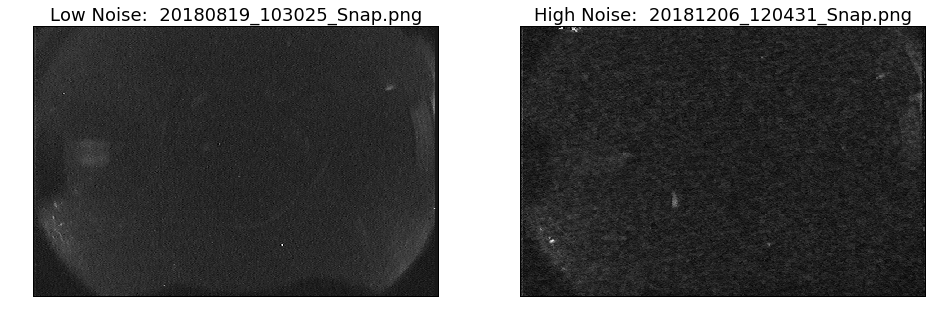
\includegraphics[scale=0.5]{images/low_and_high_noise.png}
  \caption{A D6 snapshot comparison of low and high noise.}
  \label{camera_noise}
\end{figure}

Not only was the camera noise problematic for photometric analysis, but it also made star recognition more difficult.
In a majority of the snapshots captured by the D6 AllSky Camera, we were unable to recognize any celestial objects.
A lower-noise level would allow us to recognize more stars which would add to our star catalog, and increase the number of data points used to determine observable area.
There is also a chance that we could detect dimmer stars with less-noisy data, leading to a stronger understanding of our camera's capabilities.

\section{Outlook}

Moving forward, the most important thing to focus on is data collection.
Once the problem with unusually high volumes of systematic noise is dealt with, we will have most of the framework established to create a running fireball catalog.
However, we will need to create a script that estimates a fireball's properties (energy, mass, size) given the photometry program's outputted light curve.
This project however should be fairly straightforward and will utilize the equations described in this papers background chapter.

While a singular camera can serve an important role in fireball research, systems with multiple cameras stationed in different locations have certain benefits.
They allow for the triangulation of a given fireball which can then lead to stronger velocity and position estimates.
With multiple systems, we could also estimate a fireball's orbital procession.
Next year, we hope to construct another D6 AllSky camera that will lead to more precise data collection. 
The prospect of a secondary system is exciting and will hopefully help prove that the D6 AllSky camera is a desirable alternative in fireball research.

%\input{appendix.tex}

%\bibliographystyle{urcsbiblio}
%\bibliographystyle{amsalpha}
%\bibliography{thesis_bib}
\printbibliography

%\appendix
%\include{notebook}

\end{document}
